\documentclass{beamer}
 
\usepackage[utf8]{inputenc}
\usepackage{listings}

\usepackage{algorithm}
\usepackage[noend]{algpseudocode}
\usepackage{listings}
\usepackage{color}
\usepackage{enumitem}
\usepackage{hyperref}
\usepackage{tikz}
\usetikzlibrary{positioning}

\makeatletter
\def\BState{\State\hskip-\ALG@thistlm}
\makeatother

\definecolor{dkgreen}{rgb}{0,0.6,0}
\definecolor{gray}{rgb}{0.5,0.5,0.5}
\definecolor{mauve}{rgb}{0.58,0,0.82}

\lstset{frame=tb,
  language=C++,
  aboveskip=3mm,
  belowskip=3mm,
  showstringspaces=false,
  columns=flexible,
  basicstyle={\small\ttfamily},
  numbers=left,
  numberstyle=\tiny\color{gray},
  keywordstyle=\color{blue},
  morekeywords={vector},
  commentstyle=\color{dkgreen},
  stringstyle=\color{mauve},
  breaklines=true,
  breakatwhitespace=true,
  tabsize=3
}



\definecolor{lmugreen}{RGB}{50,55,44}
 
\setbeamercolor{title}{fg=lmugreen}
\setbeamercolor{titlelike}{fg=lmugreen}
%\setbeamertemplate{itemize items}[circle]
\setbeamertemplate{itemize items}{\color{black}$\blacktriangleright$}
%\setbeamertemplate{footline}[frame number]

\setbeamertemplate{footline}[text line]{%
  \parbox{\linewidth}{\vspace*{-8pt}balken\hfill\insertshortauthor\hfill\insertframenumber/\inserttotalframenumber}}
\setbeamertemplate{navigation symbols}{}

 
%Information to be included in the title page:
\title{balken: a modern C++ barcode detection
library using mathematical morphology}
\subtitle{Praktikumsabschlusspräsentation}
\author{Tobias Heider}
\institute{Institut für Informatik, LMU M\"unchen}
\date{12.10.2018}
 
\usebackgroundtemplate%
{%
    \includegraphics[width=\paperwidth,height=\paperheight]{images/bg-empty.pdf}%
}
\setbeamertemplate{frametitle}[default][center]
 
\begin{document}
 
\frame{\titlepage}

\begin{frame}
\frametitle{Anwendung}
\centering
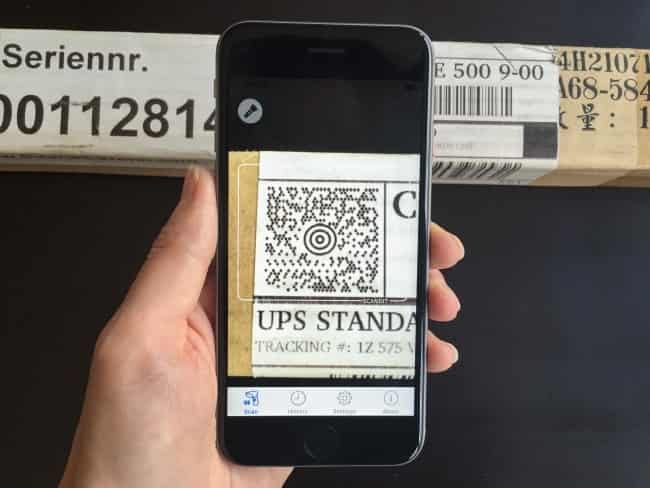
\includegraphics[width=5cm,height=3.5cm]{images/smartphone}
\begin{columns}[t]
\column{.5\textwidth}
\centering
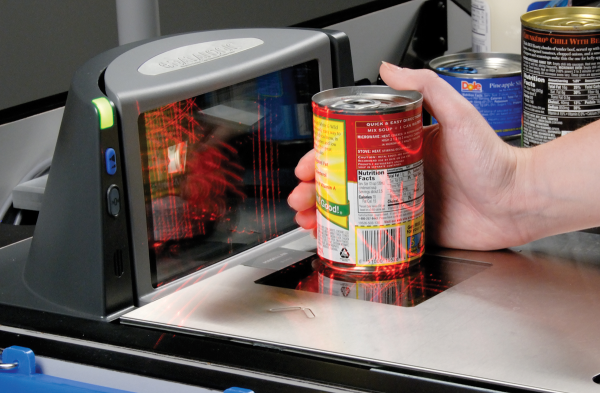
\includegraphics[width=5cm,height=4cm]{images/kasse} \\
\column{.5\textwidth}
\centering
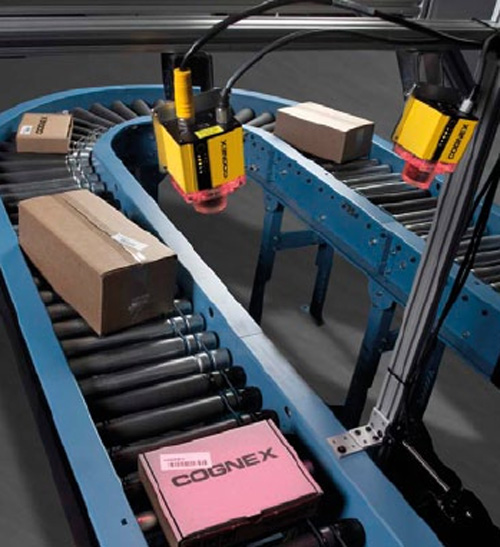
\includegraphics[width=5cm,height=4cm]{images/conveyor}
\end{columns}
\end{frame}
 
\begin{frame}
  \frametitle{Zielsetzung:}
  \begin{itemize}
    \renewcommand{\labelitemi}{--}
  \item \textbf{Echtzeitfähigkeit:} Eingaben müssen schnell genug abgearbeitet werden,
    Überschreitung von Zeitschranken richtet u.U. Schaden an.
  \item \textbf{Anpassbarkeit:} Anpassbarkeit an heterogene Hardware und Setups.
  \item  \textbf{Performance:} Niedriger Durchsatz kostet Zeit und damit oft Geld.
  \end{itemize}

\end{frame}

\begin{frame}
  \frametitle{Barcode detection}
  \begin{tikzpicture}
\node (old) {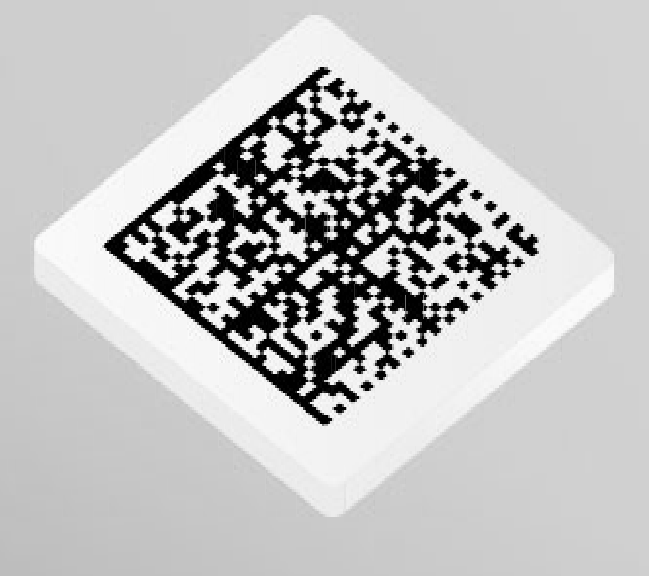
\includegraphics[width=4cm]{images/full}};
\node (good) [above right=-2cm and 1cm of old] {
\includegraphics[width=4cm]{images/diff}};
\node (background) [below right=-2cm and 1cm of old] {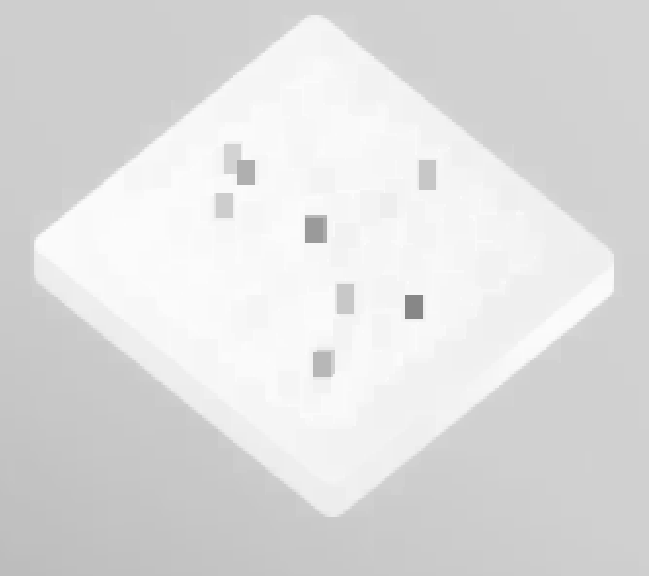
\includegraphics[width=4cm]{images/background}};

%\node (b) [fill=yellow!20,draw] at (good.center) {This is good};
\draw [ultra thick,magenta,->] (old) to[bend left] (good);
\draw [ultra thick,magenta,->] (old) to[bend right] (background);
\end{tikzpicture}
\end{frame}

% \begin{frame}
% \frametitle{Morphologie}
% \begin{columns}[t]
% \column{.5\textwidth}
% \centering
% \textbf{Erosion}
% 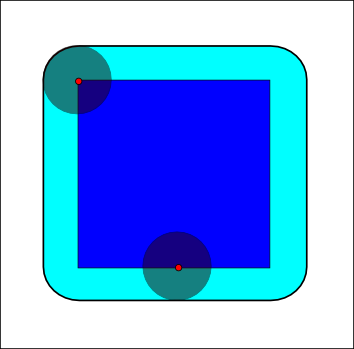
\includegraphics[width=5cm,height=5cm]{images/dilation}
% \[ A \ominus B = \bigcap_{b \in B} A_{-b} \]
% \column{.5\textwidth}
% \centering
% \textbf{Dilation}
% 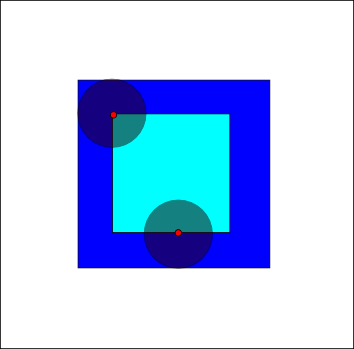
\includegraphics[width=5cm,height=5cm]{images/erosion}
% \[A \oplus B = \bigcup_{b \in B} A_{b}\]
% \end{columns}
% \end{frame}
% 
% \begin{frame}
% \frametitle{Morphologie}
% \begin{columns}[t]
% \column{.5\textwidth}
% \textbf{Opening}
% \centering
% 
\includegraphics[width=4cm,height=4cm]{images/opening}
% \[ A \circ B = (A \ominus B) \oplus B \]
% \column{.5\textwidth}
% \centering
% \textbf{Closing } %Achtung tragendes leerzeichen
% 
\includegraphics[width=4cm,height=4cm]{images/closing}
% \[ A \bullet B = (A \oplus B) \ominus B \]
% \end{columns}
% \end{frame}
% 
% \begin{frame}
%   \frametitle{Morphologie}
% \textbf{Bottom-hat transform:} 
%   \begin{tikzpicture}
% \node (background) {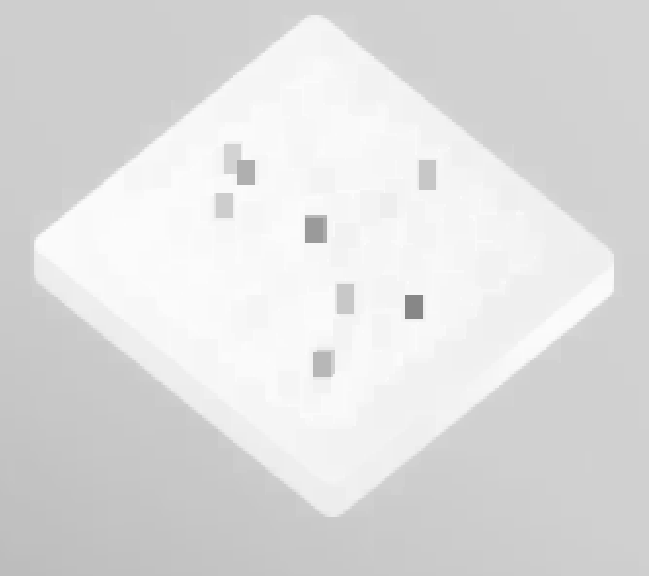
\includegraphics[width=3cm]{images/background}};
% \node (old) [right=1cm of background] {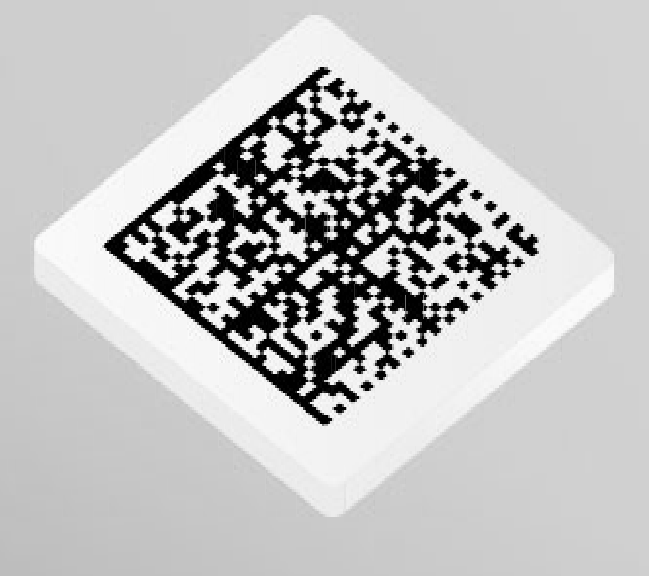
\includegraphics[width=3cm]{images/full}};
% \node (good) [right= 1cm of old] {
\includegraphics[width=3cm]{images/diff}};
% 
% %\node (b) [fill=yellow!20,draw] at (good.center) {This is good};
% \draw [ultra thick,magenta,->] (old) to (good);
% \draw [ultra thick,-] (old) to[bend] (background);
% \end{tikzpicture} \\
% \[ T_b(A) = A \bullet B - A \]
% \end{frame}
% 
% \begin{frame}
%   \frametitle{Modell}
%   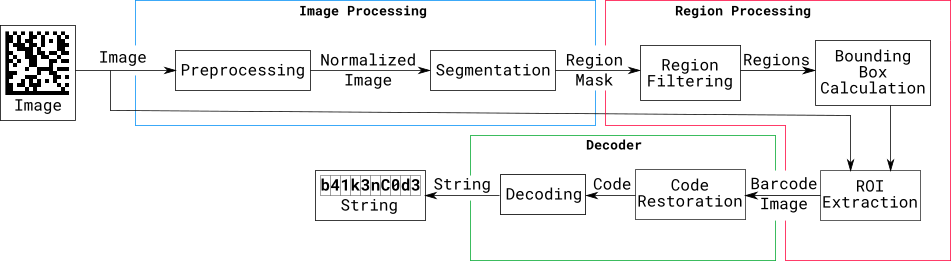
\includegraphics[width=1\textwidth]{images/systemdiagram-corner} \\
%   
%     \textbf{Image:} Konzept der Bilderverarbeitung
%     \begin{itemize}
%     \item \textbf{Expressions:} \\
%       \(Image \leftarrow load\_image(Filepath)\) \\
%       \(Image \ominus SE \equiv dilate(Image, SE)\) oder \(Image |
%         dilate(SE) \) \\
%         \(Image \bullet SE \equiv Image | dilate(SE) | erode(SE) \) \\
%         \( find\_regions(Image) \rightarrow Regions \)
%         
%     \end{itemize}
% \end{frame}
% 
% \begin{frame}
%   \frametitle{Modell}
%   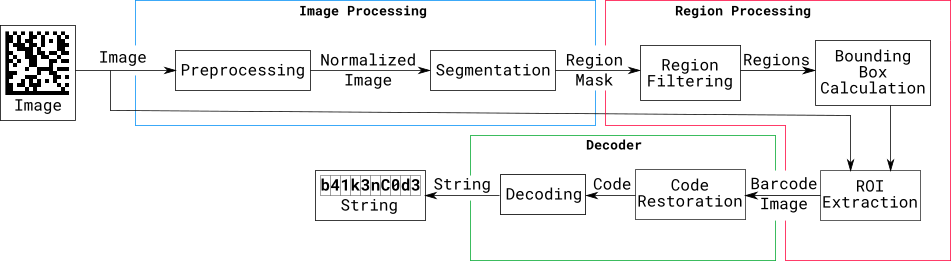
\includegraphics[width=1\textwidth]{images/systemdiagram-corner} \\
%   
%     \textbf{Region/Shape:} Konzepte der Regionsverarbeitung
%     \begin{itemize}
%     \item \textbf{Expressions:} \\
%       \(Regions \leftarrow find\_regions(Image) \) \\
%       \(convex\_hull(Region) \rightarrow Shape \) \\
%       \(bounding\_box(Region) \rightarrow Shape \) \\
%       \(extract\_shape(Image, Shape) \rightarrow Code \)
%     \end{itemize}
% \end{frame}

\begin{frame}
  \frametitle{Modell}
  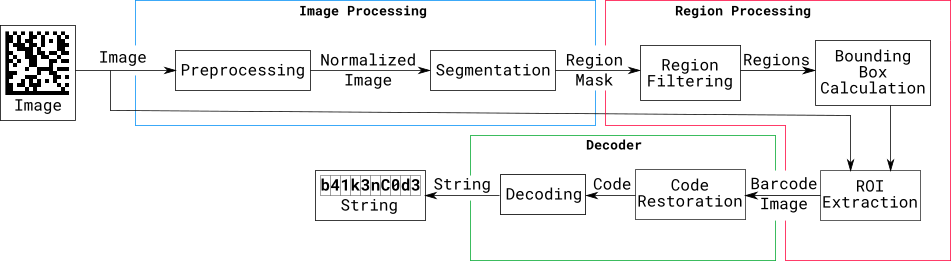
\includegraphics[width=1\textwidth]{images/systemdiagram-corner}
\end{frame}

\begin{frame}
  \frametitle{Konzepte}
  \textbf{Image:} 2-Dimensionales Bild \\~\\
  \begin{tabular}{l | l | l}
    Expression  &  Notes & Explanation \\
    \hline
    I(i,j) & \(0 <= i < I.rows()\)  and & Element Access \\ 
           & \(0 <= j < I.columns()\)   & \\
    \hline
    I.rows() &                          & Number of rows \\
    I.columns() &                       & Number of columns \\
    \hline
    \(dilate(I, SE) & \lstinline{I | dilate(SE)} & Dilation \\
    \(stretch(I)  &                              & Histogram stretch \\
    rotate(I)     &                              & Rotate Image \\
    ...           & ...                          & ... \\
    \hline
    regions::find(I) &                              & Find coherent foreground \\
                                                  & & regions
  \end{tabular}
\end{frame}

\begin{frame}
  \frametitle{Konzepte}
  \textbf{Region:} Menge von zusammenhängenden Bildpunkten \\~\\
  \begin{tabular}{l | l | l}
    Expression  &  Explanation \\
    \hline
    STL Container & Fullfills STL Container concept \\
    \hline
    dimensions(R)   & Dimensions of the Region \\
    bounding\_box(R) & Minimal bounding box contour \\
    convex\_hull(R) & Convex hull contour \\
  \end{tabular}
  \\~\\
  \textbf{Contour:} Umriss einer Region \\~\\
  \begin{tabular}{l | l | l}
    Expression  &  Explanation \\
    \hline
    Region & Fullfills Region concept \\
    \hline
    draw\_contour(I, R) & Draw contour outline to image \\
    convex\_hull(R)  & Convex hull contour \\
    subimage(I, R)   & Get view on subimage defined by shape
  \end{tabular}
  \hline
\end{frame}

\begin{frame}[fragile]
\frametitle{Implementierung}
\begin{lstlisting}[caption=Basis Klasse zur Konstruktion von Views]
template <class ImageT, class ViewT>
class ViewBase {

  constexpr ViewBase(const ImageT & img) : _img{img} {}

  // Element Access
  constexpr decltype(auto) operator()(const size_t i, const size_t j) const {
    return derived().view_element(i, j);
  }

protected:
  const ImageT & _img;
};
\end{lstlisting}
\end{frame}
  
\begin{frame}[fragile]
\frametitle{Implementierung}
\begin{lstlisting}[caption=BinaryView mittels ``Thresholding'']
template <class ImageT>
class BinaryView : public view::ViewBase<ImageT, BinaryView<ImageT>> {

  // Element Access
  constexpr ElementType view_element(std::size_t    i,
                                     std::size_t    j) const {
    return this->_img(i, j) > _threshold ? 255 : 0;
  }

private:
  const uint8_t _threshold;
};
\end{lstlisting}

\end{frame}

\begin{frame}
\frametitle{Referenz Implementierung}

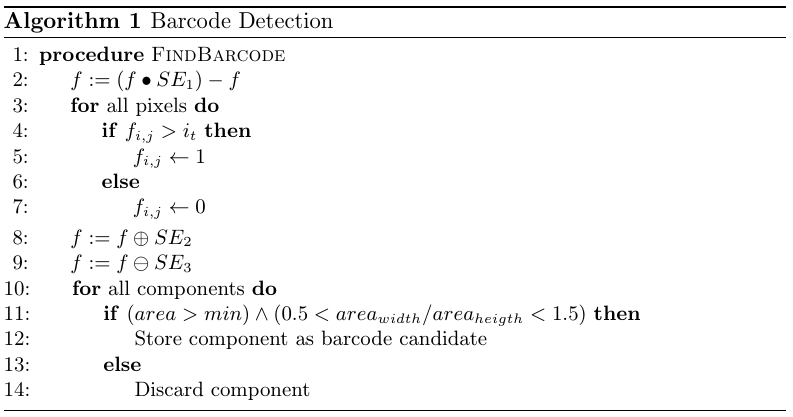
\includegraphics[width=\textwidth]{images/algorithm}
  
\end{frame}

\end{document}